% !TEX root = ../thesis.tex

\chapter{Vyhodnotenie}\label{ch:evaluation}
\section{Matematické pozadie}\label{ch:problem}
\subsection{Konečné polia}

Prejdime k základom matematiky, konkrétne k definícii základov konečných polí a k tomu, čím sa líšia od skupín.
najprv prejsť k základom konečných polí, polí vo všeobecnosti a
skupín.
Skupina je množina prvkov spolu s operátorom, ktorý kombinuje ľubovoľné dva prvky skupiny a vytvára tretí prvok. Tento operátor musí spĺňať štyri podmienky, známe aj ako axiómy grupy:

\begin{itemize}
	\item Uzavretosť: všetky vytvorené prvky sú tiež v skupine.
	\item Asociatívnosť: ∀a, b, c: (a ◦ b) ◦ c = a ◦ (b ◦ c), kde ◦ je použitý operátor.
	\item  Identita: existuje prvok Id taký, že ∀a: (a ◦ Id = a).
	\item Invertibilita: každý prvok a v skupine má inverziu, takže
	a ◦ a-1 = Id.
\end{itemize}

Ak okrem toho spĺňa rovnicu komutatívnosti a◦b = b◦a,
nazýva sa abelická grupa. V prípade kombinácie množiny celých čísel
s operátorom +, ◦ = +, Id = 0 a a-1 = -a, pretože a + b = b + a,
je to tiež abelovská grupa.

Konečné pole Fp, nazývané aj Galoisovo pole, používané v eliptickej krivke
je pole s konečným počtom prvkov. Rád p
poľa je počet prvkov v ňom. Pole je abelovská grupa s
sčítaním a ďalším operátorom, a to násobením. Sčítanie spĺňa
všetky podmienky z abelických skupín. Násobenie je uzavreté, asociatívne
a komutatívna rovnako ako sčítanie. Okrem toho má
vlastný neutrálny prvok 1, kde 1 - a = a - 1 = a pre nejaký prvok
a. Každý prvok okrem 0 má inverzný prvok aj pre násobenie,
a - a-1 = a-1 - a = 1. Napokon, násobenie je distribučné s
vzhľadom na sčítanie, t. j. ∀a, b, c: (a - (b + c) = a - b + a - c).

\subsection{Elliptic curves}

Nech \( F \) je pole a \( E \) je krivka definovaná nad týmto poľom \( F \). Množina riešení \( E(F) \) pre nasledujúcu všeobecnú rovnicu je:

\[
y^2 = x^3 + ax^2 + bx + c
\]

kde \( a, b, c \in F \).

Pre nás sú zaujímavejšie Montgomeryho krivky, pretože sa používajú v NaCl knižnici. Všeobecne platí, že Montgomeryho krivky vyžadujú menej kódu a sú odolnejšie voči časovým útokom v porovnaní s bežnými eliptickými krivkami \cite{OKS00}. 

Montgomeryho krivka \( E \) má tvar:

\[
E(F_p) = \{\infty\} \cup \{(x, y) \in F_p : B y^2 = x^3 + Ax^2 + x \}
\]

kde \( \infty \) predstavuje "bod v nekonečne", ktorý slúži ako identita, a \( A \) je veľké celé číslo, pričom platí \( A^2 - 4 \neq \text{štvorec modulo} \, p \). Táto krivka by nemala mať žiadne vrcholy (ostrý bod) ani vlastné priesečníky, čo je dôležité, pretože potrebujeme krivku, ktorá je diferencovateľná (krivka s vrcholmi nemá jedinečnú deriváciu v bode vrcholu).

Následne môžeme definovať operáciu sčítania na tejto krivke, aby sme mohli implementovať kryptografické operácie. Spolu s bodom nekonečna tvoria body na krivke abelickú skupinu.

	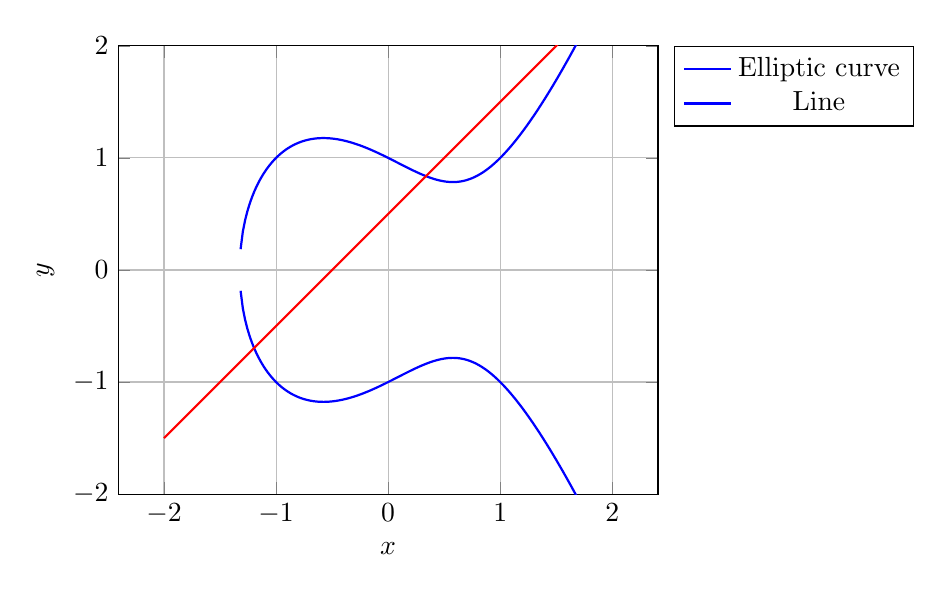
\begin{tikzpicture}
		\begin{axis}[
			axis equal,
			xlabel={$x$},
			ylabel={$y$},
			domain=-2:2,
			samples=100,
			grid=major,
			xmin=-2, xmax=2, ymin=-2, ymax=2,
			legend pos=outer north east
			]
			
			% Normalized elliptic curve y^2 = x^3 - x + 1
			\addplot [
			blue,
			thick,
			samples=200,
			domain=-2:2,
			] ({x}, {sqrt(x^3 - x + 1)});
			
			\addplot [
			blue,
			thick,
			samples=200,
			domain=-2:2,
			] ({x}, {-sqrt(x^3 - x + 1)});
			
			% Line intersecting the curve
			\addplot [
			red,
			thick,
			domain=-2:2,
			] {x + 0.5};
			
			\legend{Elliptic curve, Line}
			
		\end{axis}
	\end{tikzpicture}


Začneme s binárnym operátorom \( + \), ktorý môžeme najjednoduchšie opísať slovami: zoberte rôzne body \( A \) a \( B \), ktoré chceme sčítať, a nakreslite priamku cez tieto body. Existuje presne jeden ďalší bod priesečníka na krivke. Vypočítajte, kde sa nachádza tento tretí bod, a potom ho odrazte o os \( x \). 

„Dvojnásobenie“ bodu sa vykonáva tak, že vezmeme dotyčnicu v bode \( A \), potom vypočítame druhý bod priesečníka a vezmeme negáciu tohto bodu. Ak je priamka paralelná k osi \( y \), vezmeme identitný prvok \( \infty \). Na základe toho môžeme definovať operáciu \( + \) nasledovne: \\ \\
1. \( \infty + \infty = \infty \) \\
2. \( \infty + (x, y) = (x, y) + \infty = (x, y) \) \\
3. \( (x, y) + (x, -y) = \infty \) \\
4. Ak \( y \neq 0 \), potom \( (x, y) + (x, y) = (x'', y'') \), kde \( x'' = \lambda - A - 2x = \frac{(x^2 - 1)^2}{4y^2} \) a \( y'' = \lambda(x - x'') - y \). \( \lambda \) označuje prvú deriváciu \( E \), pričom \( \lambda = \frac{3x^2 + 2Ax + 1}{2y} \). (Dvojnásobenie bodu) \\
5. Ak \( x \neq x' \), potom \( (x, y) + (x', y') = (x'', y'') \), kde \( x'' = \Delta^2 - A - x - x' \) a \( y'' = \Delta(x - x'') - y \). Tu je \( \Delta \) definované ako \( \Delta = \frac{y' - y}{x' - x} \), inými slovami, je to sklon funkcie medzi bodmi \( (x, y) \) a \( (x', y') \). (Sčítanie) \\

Sčítanie identitného prvku a iného prvku \( X \) vedie k \( X \), ako je vidieť v (1) a (2). Sčítanie bodu a jeho negácie tiež vedie k identitnému prvku (3). V (4) sa dvojnásobenie bodu vykonáva najskôr výpočtom prvej derivácie, potom vypočítaním dotyčnice a vzatím negácie \( y \). V prípade, že \( y = 0 \), platí \( (x, 0) + (x, 0) = \infty \). (5) definuje „normálne“ sčítanie, kde vezmeme sklon medzi dvoma priamkami \( \Delta \) a vypočítame tretí bod \( x'' \). Ak \( x = x'' \), potom bude platiť (4). 


Sčítanie identitného prvku a iného prvku \( X \) vedie k \( X \), ako je vidieť v (1) a (2). Sčítanie bodu a jeho negácie tiež vedie k identitnému prvku (3). V (4) sa dvojnásobenie bodu vykonáva najskôr výpočtom prvej derivácie, potom vypočítaním dotyčnice a vzatím negácie \( y \). V prípade, že \( y = 0 \), platí \( (x, 0) + (x, 0) = \infty \). (5) definuje „normálne“ sčítanie, kde vezmeme sklon medzi dvoma priamkami \( \Delta \) a vypočítame tretí bod \( x'' \). Ak \( x = x'' \), potom bude platiť (4). Na obrázku 1b môžeme vidieť dvojnásobenie bodu, zatiaľ čo na obrázku 1a môžeme vidieť sčítanie.

\subsection{Eliptické krivky nad \( F_p \)}

Uvedená aritmetika je pomalá a nie je vhodná na kryptografické účely, pretože potrebujeme nekonečný počet bodov. Je potrebné niečo rýchle a presné, aby sme získali konečnú skupinu pre úlohu diskrétnych logaritmov. Toho dosiahneme kombináciou eliptických kriviek a predtým spomenutých konečných polí: eliptické krivky nad \( F_p \). Táto eliptická krivka \( E(F_p) \) obsahuje všetky body \((x, y)\), ktoré spĺňajú rovnicu eliptickej krivky modulo \( p \): \( y^2 \mod p = x^3 + Ax^2 + x \mod p \). 

\begin{figure}[h]
	\centering
	\begin{tikzpicture}
		\begin{axis}[
			width=15cm, % Ширина графика
			height=15cm, % Высота графика
			axis lines=middle,
			xlabel={$x$},
			ylabel={$y$},
			xlim={-7.5:7.5}, % Ограничения по оси x
			ylim={-7.5:7.5}, % Ограничения по оси y
			xtick={-7, -5, ..., 7},
			ytick={-7, -5, ..., 7},
			grid=both,
			minor tick num=1,
			major grid style={line width=.5pt,draw=gray!50},
			minor grid style={line width=.5pt,draw=gray!20}
			]
			% Здесь мы рисуем точки
			\addplot[only marks, mark=*] coordinates {
				(1, 2)
				(3, 5)
				(4, 3)
				(5, 6)
				(6, 7)
				(7, 8)
				(0, 0)
				(2, 2)
				(4, 4)
				(6, 6)
				(3, 1)
				(5, 2)
			};
		\end{axis}
	\end{tikzpicture}
	\caption{Graf}
	\label{fig:elliptic_curve}
\end{figure}